\section{Introduction}
Artificial intelligent systems about comprehension and inference 
can be improved by incorporating commonsense knowledge as background, 
such as ice is cold, 
chewing is a subevent of eating, 
chair and table are typically found near each other, etc. 
Such commonsense facts could benefit entailment~\cite{dagan2009recognizing}, grounded entailment~\cite{bowman2015large}, or visual recognition tasks~\cite{zhu2014reasoning}.
Such commonsense knowledge is often represented as relation triples
between two concepts or objects in ConceptNet, 
such as (\textit{ice, \textsc{HasProperty}, cold}), 
(\textit{eating, \textsc{HasSubevent}, chewing}), 
(\textit{chair, \lnear, table}) etc. 

However, commonsense knowledge such as the above is largely manually curated
or crowdsourced by community efforts and thus does not scale well.
For example, ConceptNet\footnote{\url{http://conceptnet.io/}} by MIT \cite{speer2012representing}, one of the largest commonsense
knowledge graph available today, contains only 49 \lnear~
relation triples. 
Many commonly co-located objects such as (house, garden) and 
(fork, knife) are not included in this knowledge base. 
Another problem with manually curated data source is that, because manual
annotation is expensive, a fact is typically contributed by just one 
or a few persons. 
As a result, no meaningful statistical confidence scores can be
associated with each triple, which makes rank-based 
computation using such knowledge base difficult. 
For instance, although ConceptNet gives a confidence
score (from 0 to infinity) to each triple, most of the triples have the default
score of 1, simply because the human contributor did not or could not 
provide a score. 
If such commonsense knowledge is harnessed automatically
from open-domain text corpora, both of the above problems can be 
effectively addressed. 
Open information extraction not only provides the much needed scale,
but also valuable statistics that can turn into confidence scores.

\begin{figure}[th]
\center
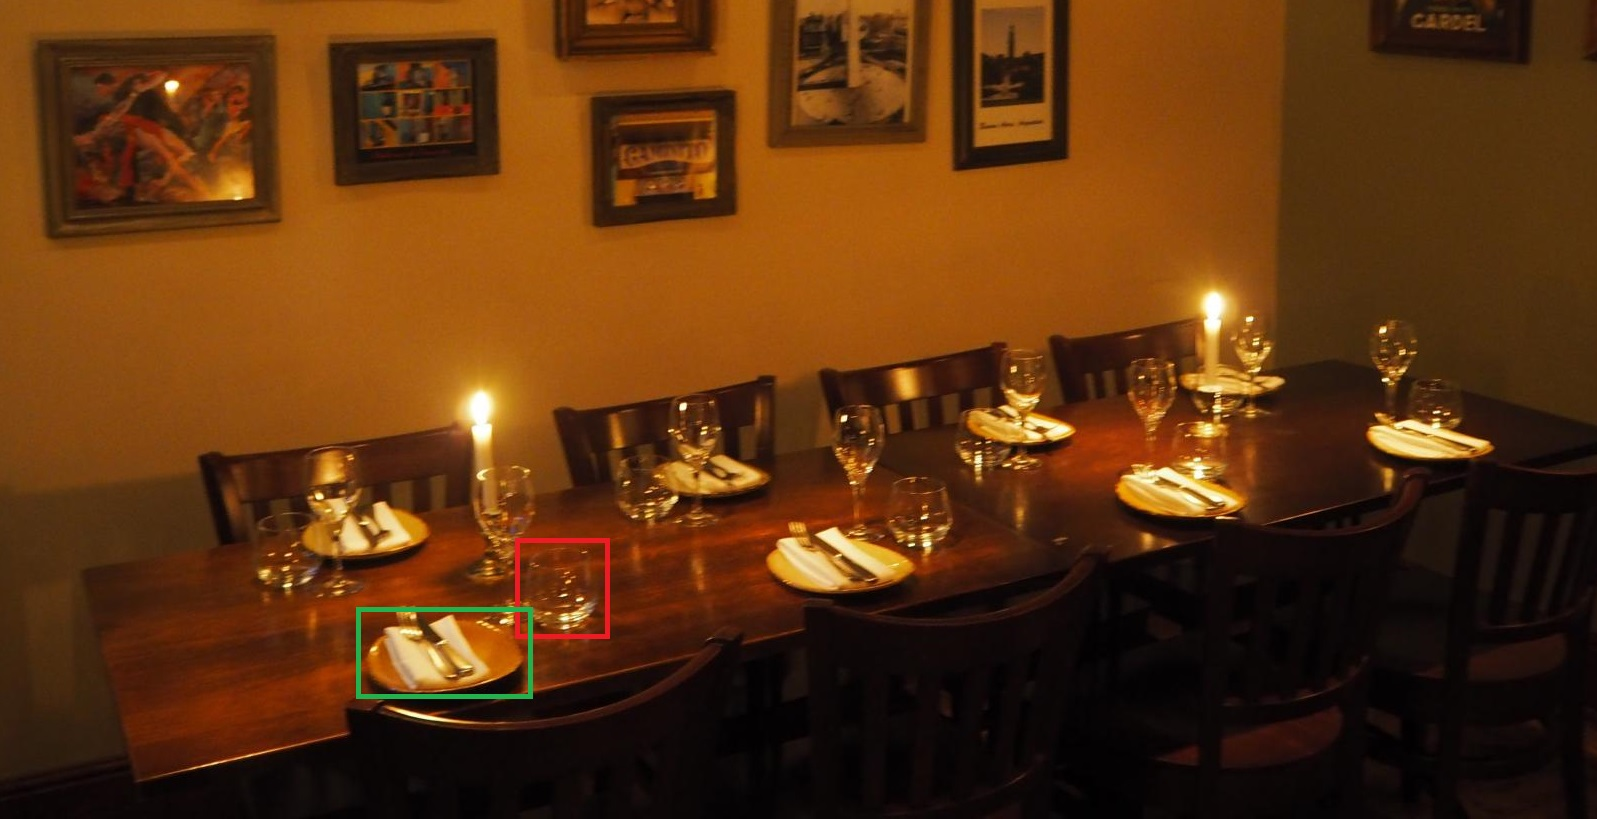
\includegraphics[width=\columnwidth]{dim-table.jpg}
\caption{A dimly lit room with a dining table, plates and glasses}
\label{fig:dim}
\end{figure}

In this paper, we want to extract the \lnear\ relation between
phyical objects, which is defined as two objects typically found near each
other.\footnote{Because some physical objects can be a location itself, this
relation may include some instances of the \textsc{atLocation} relation,
e.g., {\em room} and {\em door}.}
We focus on \lnear\ relation for these reasons:
\begin{itemize}
	\item Prior knowledge of \lnear\ relations is helpful for object detection in complex image scenes. 
	For example, in a dimly lit restaurant, if some plates are present on a table,
	One may guess that wine glasses or other kitchenware maybe nearby, 
	even though these objects are hardly visible (see \figref{fig:dim}). 
	%Such prior knowledge helps with the object detection accuracy; 
	\item \lnear~ relation can benefit general reasoning in reading comprehension,
	question answering and many other AI tasks;
	\item Existing knowledge bases such as ConceptNet has very limited facts for
	this relation.
\end{itemize} 


%
%\begin{enumerate}
%\item \lnear relation is useful for object detection in complex image 
%scenes. For example, in a dimly lit room with a dining table and some chairs.
%One may guess that plates and other kitchenware maybe present on the table.
%Such prior knowledge helps with the object detection accuracy. \KZ{give a 
%real image here which is hard to detect by state-of-the-art algo but 
%obeys commonsense.}
%
%%\item \lnear relation can also be useful for automated conversation systems
%%where meaningful context maybe added to the conversation. \KZ{Example?}
%
%\item \lnear relation can benefit general reasoning in reading comprehension,
%question answering and many other AI tasks.
%
%\item Existing knowledge bases such as Concept Net has very limited facts for
%this relation.
%\end{enumerate}

Automatic extraction of relations from open text has a short but rich history. 
Attempts have been made to extract isA, causal, correlation, and 
also open domain relations (e.g., ReVerb, Yago).
%\KZ{cite and Say more about KBC}. 
\lnear~relation is unique and poses significant challenges
for the following reasons:
\begin{itemize}
	\item It involves physical (often visible) objects whereas other 
	popular relations involve general concepts or just natural language terms. 
	
	\item The distribution of \lnear~ relation is not even across domains: 
	it is more prevalent in literary work such as stories 
	and dramas which come with descriptive scenes rather
	than in news, science \& technology related articles or online user 
	generated content. 
	%Our preliminary investigation shows that XXX\% of the sentences 
	%in New York Times and YYY\% of the sentences
	%in Wikipedia contains a \lnear~ relation, 
	%while that percentage for novels and stories in Gutenberg corpus is ZZZ\%. 
	
	\item Sentences in literature are often complex and nuanced, 
	which makes extraction particularly challenging. Consider the objects
	``bed'' and ``star'' in the following
	sentence: ``{\em Until at last all the promenaders had gone home to bed, 
	and I was alone with the star.}'' Bed is not near the star because it's at another location.
	
	\item Labeling such sentence is a non-trivial task, 
	and obtaining a large training set is difficult and expensive.
\end{itemize}

%\BL{add more related work about KBC here, mainly about Xiang Li (TTIC) and Stating the Obvious; to stress that why we are using raw text}

%Since raw text of novels tend to contain many 
%descriptions of  scene in real life, 
%we argue that it is feasible to obtain unseen 
%{\lnear} relations from raw novel text. 

In this paper we propose two tasks in solving \lnear\ relation
extraction problem. One is a binary classification problem which detects
two {\em co-located} physical objects in a sentence. 
The other one is given result of the above classification on
large number of sentences, how to produce a ranked list of \lnear\
facts as a knowledge base. Each \lnear\ fact carries a confidence weight
that indicates the typicality of the fact given the evidence from the
text corpus. Notice that two objects that are {\em co-located} 
in a couple of sentences may not mean they have 
the \lnear\ relation as a commonsense. This confidence weight can serve
as a smoothed version of the confidence score in ConceptNet.

To this end, we created two 
benchmark datasets, one with 5,000 sentences, 
each containing at least two physical objects,
and a label of co-location or not; the other consisting of 500 pairs of
objects with binary labels, that is whether a pair is \lnear\ or not.  

%is to build a framework to automatically extract 
%large amount of unseen object pairs with \lnear relations 
%from literary text corpora.
%that 
%are not already included in ConceptNet. \KZ{Need to back up this claim in eval}
%Considering the fact that not all sentences mentioning two physical objects 
%indicate that the two objects are nearby each other, 
%our proposed approach is to first construct a sentence-level relation classification model 
%to identify \lnear~ relation and then score each candidate object pair with the model 
%and the sentences containing it.
%Thus, the core problem is to judge whether a given sentence 
%containing two objects is describing a \lnear~ relation between the two objects or not. 
%

%More formally, given a sentence $s$ mentioning a pair of physical objects 
%\textless$e_1,e_2$\textgreater, 
%the problem is to determine whether $e_1$ and $e_2$ are located near each other in a physical scene 
%described in the sentence $s$. 
%
%\begin{table}[th!]
%	\centering
%	\caption{Examples for sentence-level \lnear Classification; The  \textless$e_1,e_2$\textgreater in both instances is \textless dog,cat\textgreater. Since the the first sentence is describing a physical scene about the dog and the cat, 
%		while the dog and the cat in the second sentence do not have to be located near since it is just talking about a general comparison.}
%	\label{tbl:lnc}
%	\begin{tabular}{|c|c|}
%		\hline
%		$s$    &  T/F\\ \hline
%	My dog is older than her cat.	 &  T\\ \hline
%	The King put his dog and cat on the table.     & F  \\ \hline
%	\end{tabular}
%
%\end{table}
%
%\KZ{Can use the two examples earlier. 
%For example, suppose $s_1$ = ``The King put his dog and cat on the table.'', 
%$s_2$ = ``My dog is older than her cat.'', 
%$e_1$ is ``dog" and $e_2$ is ``cat''. 
%Then the answer of $s_1$ is \textit{True} and of  $s_2$ is \textit{False} , 
%since the $s_1$ is describing a physical scene about the dog and the cat, 
%while the dog and the cat in $s_2$ do not have to be located near since it is just talking about a general comparison.
%}

%\BL{Add related work here about the relation classification , and their shortcoming (too many parameters) }

We also propose two baseline methods to solve the classification task.
The first approach leverages syntactic features and word embedding
in the sentence in a SVM model. The second approach is an LSTM
model that takes advantage of word embeddings of the 
two objects and the most relevant sequential information of the sentences 
indicating the co-location, significantly reducing the size of 
parameters. In both approaches,
we associate a probabilistic score with each pair of objects extracted
from a sentence. We then aggregate such scores for each unique pair,
to produce a commonsense knowledge score for this pair.  
%We construct a dataset consisting of \BL{xxx} instances with labels 
%(\textit{True}/\textit{False}) for training our model. 
%Experiments demonstrate that both of the classification methods 
%outperforms the state-of-art approaches on the \lnear dataset.
%\KZ{Need to back up these in the eval.} 

In summary, this paper makes the following contributions:

\begin{itemize}
	\item We proposed two novel tasks for \lnear~ relation extraction
	(\secref{sec:method}).
	
	\item We make public the first annotated dataset for 
	sentence-level \lnear~ relation classification and another labeled dataset for
	\lnear~ knowledge construction (\secref{sec:data}). 
	%	\item We propose a bootstrapping framework that automatically generate X times more training data than the initially labeled.
	
	\item We suggest several baseline methods for \lnear~ relation 
	classification task (\secref{sec:method}), 
	which compare favorably with the current state-of-the-art
	method for general-purpose relation classification problem (\secref{sec:eval}). 
	
	\item We extract in total 2,067 new pairs previously not in
	ConceptNet, with a precision of 0.68 (\secref{sec:eval}).
\end{itemize}


